%!TEX root = draft.tex
\section{Reducing Linearizability of Priority Queues to Reachability}
\label{sec:co-regular of extended priority queues}

We show that the set of executions for which $\textit{Check-PQ-Conc-NonRec}$ fails on some projection can be described using register automata, modulo a value renaming. Renaming values (which is complete under data independence) allows to simplify the reasoning about projections. W.l.o.g., we assume that all the operations which are not in the projection failing this test use the same distinguished value $\top$, different from those in the projection. Then, it is enough to find an automata characterization of the executions $e$ for which $\textit{Check-PQ-Conc-NonRec}(e)$ is $\mathsf{false}$, i.e., for which
$\Gamma(e) := \mathsf{Has\text{-}}\Gamma(e) \Rightarrow \exists \alpha.\ \Gamma\mathsf{\text{-}Conc}(e,\alpha)$ is false, for some $\Gamma\in \{\mathsf{EmptyRemove}$, $\mathsf{UnmatchedMaxPriority}$, $\mathsf{MatchedMaxPriority}\}$.
Intuitively, $\Gamma(e)$ states that $e$ is linearizable w.r.t. the set of sequential executions described by $\Gamma\mathsf{\text{-}Seq}$ (provided that $\mathsf{Has\text{-}}\Gamma(e)$ holds). Therefore, by an abuse of terminology, an execution $e$ satisfying $\Gamma(e)$ is called \emph{linearizable w.r.t. $\Gamma$}, or \emph{$\Gamma$-linearizable}.
Extending the automaton characterizing non $\Gamma$-linearizable executions with self-loops that allow any operation with argument $\top$ results in an automaton satisfying the following property called \emph{$\Gamma$-completeness}.

\begin{definition}
For $\Gamma\in \{\mathsf{EmptyRemove}$, $\mathsf{UnmatchedMaxPriority}$, $\mathsf{MatchedMaxPriority}\}$, an automaton $A$ is called \emph{$\Gamma$-complete} when for each data-independent implementation $\mathcal{I}$:

$A \cap \mathcal{I} \neq \emptyset$ iff there exists $e \in \mathcal{I}$ and $e' \in \textit{proj}(e)$ such that $e'$ is not $\Gamma$-linearizable.
\end{definition}




We can show that for any $\Gamma\in \{\mathsf{EmptyRemove}$,$\mathsf{UnmatchedMaxPriority}$,$\mathsf{MatchedMaxPriority}\}$ there exists a $\Gamma$-complete automaton. For lack of space, we only consider the case $\Gamma=\mathsf{MatchedMaxPriority}$ in
Section~\ref{ssec:aut}.
When defining $\Gamma$-complete automata, we assume that every implementation $\mathcal{I}$ behaves correctly, i.e., as a FIFO queue, when only values with the same priority are observed. More precisely, we assume that for every execution $e\in\mathcal{I}$ and every priority $p\in\mathbb{P}$, the projection of $e$ to values with priority $p$ is linearizable (w.r.t. $\seqPQ$). This property can be checked separately using register automata similar to the automata in~\cite{DBLP:conf/icalp/BouajjaniEEH15} describing FIFO queue violations (see Appendix~\ref{sec:appendix lemma and register automata for FIFO of single-priority executions} for more details). This assumption excludes some obvious violations, such as an $\textit{rm}(a)$ operation happening before a $\textit{put}(a,p)$ operation, for some $p$.

For $\Gamma\in \{\mathsf{UnmatchedMaxPriority}, \mathsf{MatchedMaxPriority}\}$, we consider $\Gamma$-complete automata recognizing executions which contain only one maximal priority. This is w.l.o.g. because any data-differentiated execution for which $\Gamma(e)$ is false has such a projection.
Formally, given a data-differentiated execution $e$ and $p$ a maximal priority in $e$, $e\vert_{\preceq p}$ is the projection of $e$ to the set of values with priorities smaller or equal to $p$. Then,

\begin{lemma}
\label{lemma:pri execution is enough}
For $\Gamma\in \{\mathsf{UnmatchedMaxPriority}, \mathsf{MatchedMaxPriority}\}$, a data-differentiated execution $e$
 is $\Gamma$-linearizable iff $e\vert_{\preceq p}$ is $\Gamma$-linearizable for some maximal priority $p$ in $e$.
\end{lemma}
\begin {proof} (Sketch)
For the ``only-if'' direction, let $e$ be a data-differentiated execution linearizable w.r.t. $l = u \cdot \textit{put}(x,p) \cdot v \cdot \textit{rm}(x) \cdot w$ s.t. $\mathsf{MatchedMaxPriority}\mathsf{\text{-}Seq}(l,x)$ holds. Since the predicate $\mathsf{MatchedMaxPriority}\mathsf{\text{-}Seq}(l,x)$ imposes no restriction on the operations in $u$, $v$, and $w$ with priorities incomparable to $p$, erasing all these operations results in a sequential execution which still satisfies this predicate. Similarly, for $\Gamma=\mathsf{UnmatchedMaxPriority}$.

The ``if'' direction follows from the fact that if the projection of an execution to a set of operations $O_1$ has a linearization $l_1$ and the projection of the same execution to the remaining set of operations has a linearization $l_2$, then the execution has a linearization which is defined as an interleaving of $l_1$ and $l_2$ (see Appendix~\ref{sec:appendix proof of Lemma pri execution is enough} for more details).

Thus, let $e$ be an execution such that $e\vert_{\preceq p}$ is linearizable w.r.t. $l = u \cdot \textit{put}(x,p) \cdot v \cdot \textit{rm}(x) \cdot w$ where $\mathsf{MatchedMaxPriority}\mathsf{\text{-}Seq}(l,x)$ holds. By the property above, we know that $e$ has a linearization $l' = u' \cdot \textit{put}(x,p) \cdot v' \cdot \textit{rm}(x) \cdot w'$, such that the projection of $l'$ to values of priority comparable to $p$ is $l$.
Since $\mathsf{MatchedMaxPriority}\mathsf{\text{-}Seq}(l,x)$ doesn't constrain the values of priority incomparable to $p$, we obtain that $\mathsf{MatchedMaxPriority}\mathsf{\text{-}Seq}(l',\alpha)$ also holds.
\end {proof}

We shows in Appendix \ref{subsec:appendix co-regular of EPQ2Lar} and Appendix \ref{subsec:appendix co-regular of EPQ2Equal} that it is safe to ignore constructing $\mathsf{UnmatchedMaxPriority}$-complete register automata, and we give the $\mathsf{EmptyRemove}$-complete register automata in Appendix \ref{subsec:co-regular of EPQ3}. The existence of $\Gamma$-complete automata enable an effective reduction of checking linearizability of concurrent priority queue implementations to state reachability.
Section~\ref{subsec:combine step-by-step linearizability and co-regular} discusses decidability results implied by this reduction.

\begin{theorem}
\label{lemma:reduce EPQ into state reachability}
Let $\mathcal{I}$ be a data-independent implementation. Then, there is a $\Gamma$-complete automaton $A(\Gamma)$ for each $\Gamma$. Moreover,
$\mathcal{I} \sqsubseteq \seqPQ$ iff $\mathcal{I} \cap A(\Gamma) = \emptyset$ for all $\Gamma$.
\end{theorem}



\subsection{A $\mathsf{MatchedMaxPriority}$-complete automaton}\label{ssec:aut}


A differentiated execution $e$ is not $\mathsf{MatchedMaxPriority}$-linearizable when all the $\textit{put}$ operations in $e$ using the maximal priority $p$ are matched, and $e$ is not linearizable w.r.t. the set of sequential executions satisfying $\mathsf{MatchedMaxPriority\text{-}Seq}(e,x)$ for each value $x$ of priority $p$. We consider two cases depending on whether $e$ contains exactly one value with priority $p$ or at least two values. We denote by $\mathsf{MatchedMaxPriority}^{>}$ the strengthening of $\mathsf{MatchedMaxPriority}$ with the condition that all the values other than $x$ have a priority strictly smaller than $p$ (corresponding to the first case), and by $\mathsf{MatchedMaxPriority}^{=}$ the strengthening of the same formula with the negation of this condition (corresponding to the second case).
We use particular instances of register automata~\cite{DBLP:journals/tcs/KaminskiF94,DBLP:conf/icalp/Cerans94,DBLP:conf/stacs/SegoufinT11} whose states include only two registers, one for storing a priority guessed at the initial state, and one for storing the priority of the current action in the execution. The transitions can check equality or the order relation $\prec$ between the values stored in the two registers. Instead of formalizing the full class of register automata, we consider a simpler class which suffices our needs. Thus, we consider a class of labeled transition systems whose states consist of a finite control part and a register $r$ interpreted to elements of $\mathbb{P}$. The transition labels are:
\begin{itemize}
	\item $r=*$ for storing an arbitrary value to $r$,
	\item $\textit{call}(\textit{rm},a)$ and $\textit{ret}(\textit{rm},a)$ for reading call/return actions of a remove,
	\item $\textit{call}(\textit{put},d,g)$ where $g\in\{=r,\prec r,true\}$ is a guard, for reading a call action $\textit{call}(\textit{put},d,p)$ and checking if $p$ is either equal to or smaller than the value stored in $r$, or arbitrary,
	\item $\textit{ret}(\textit{put},d,true)$ for reading a return action $\textit{ret}(\textit{put},d,p)$ for any $p$.
\end{itemize}
The set of sequences (executions) accepted by such a transition system is defined as usual.





\subsubsection{A $\mathsf{MatchedMaxPriority}^>$-complete automaton}
\label{subsec:co-regular of EPQ1Lar}

\begin{figure}[t]
  \centering
  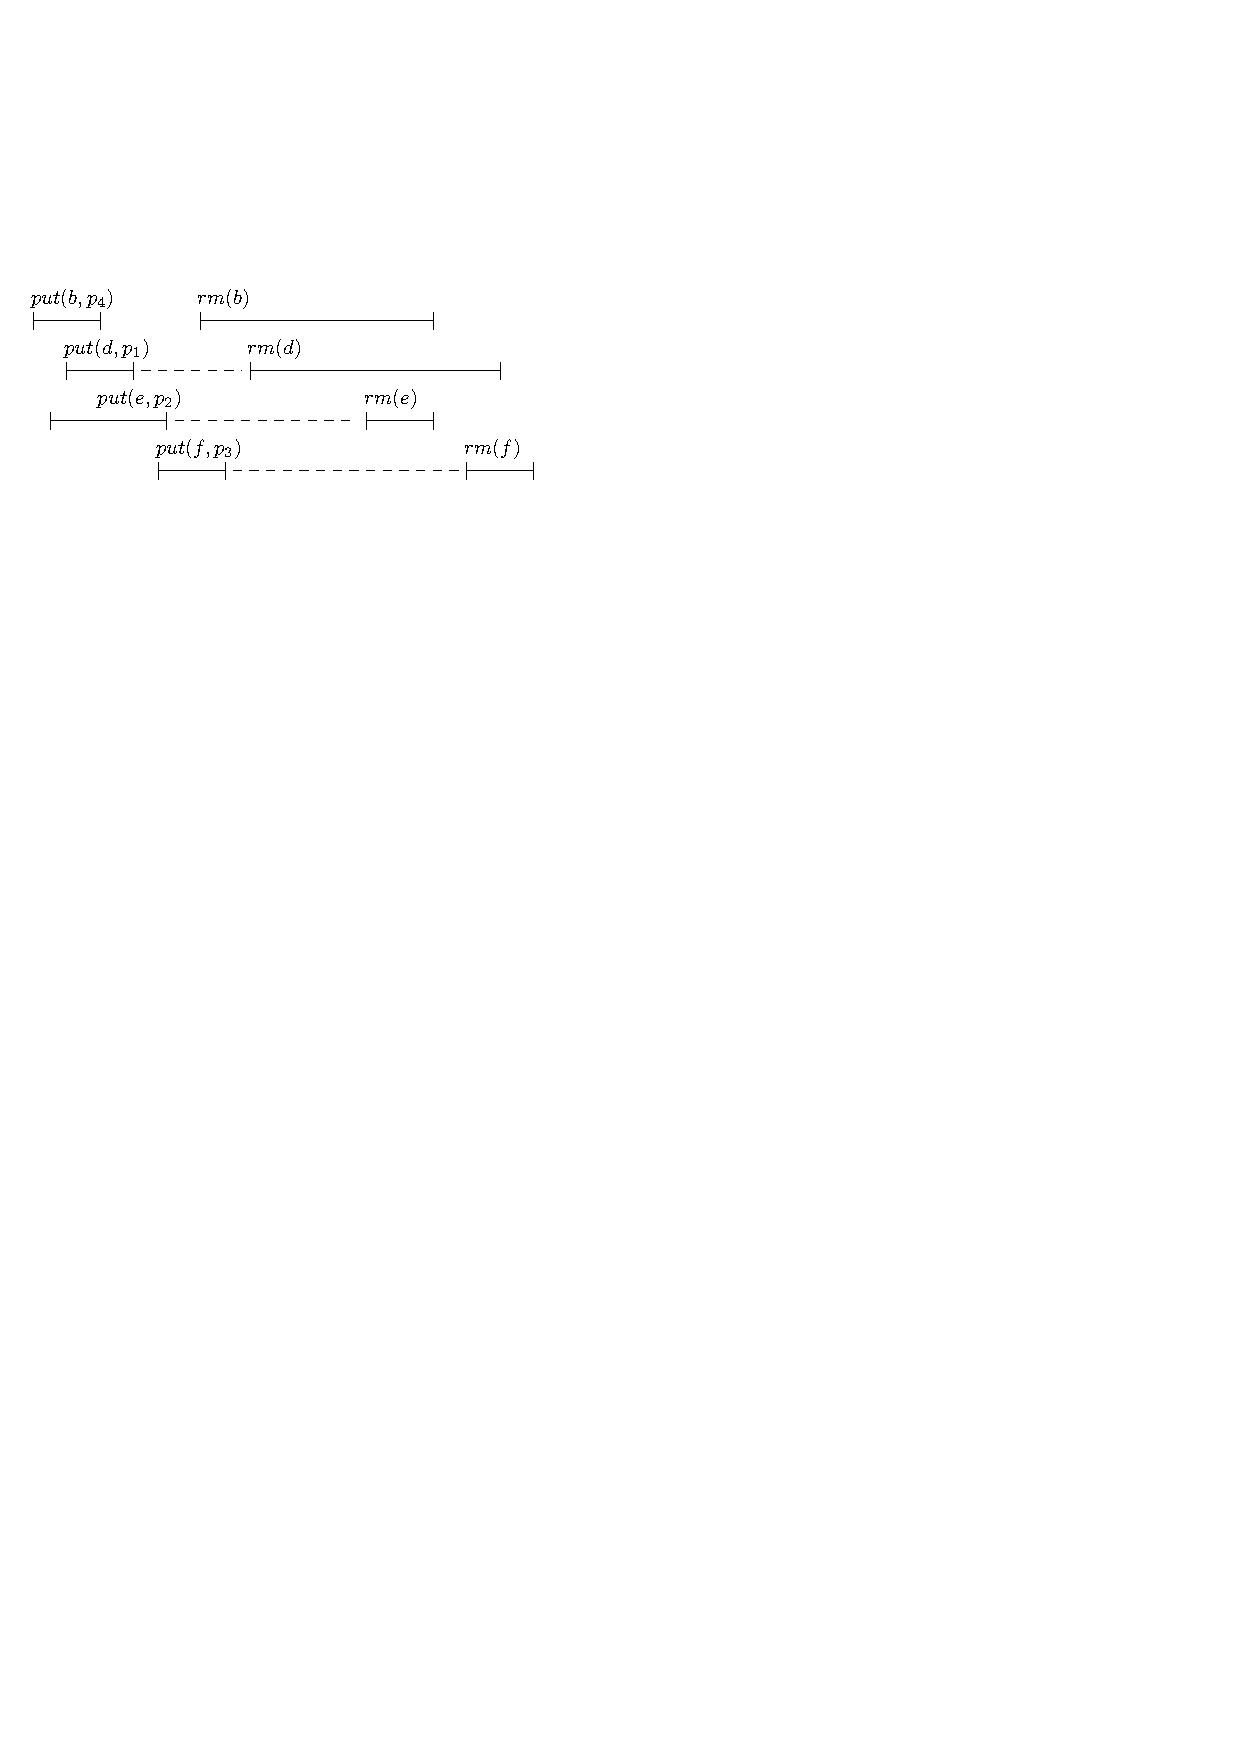
\includegraphics[width=0.4 \textwidth]{figures/PIC-HIS-INTRO-GAP-EPQ1L.pdf}
  \caption{An execution that is not $\mathsf{MatchedMaxPriority}^{>}$-linearizable. We represent each operation as a time interval whose left, resp., right, bound corresponds to the call, resp., return action.}
  \label{fig:introduce gap for EPQ1Lar}
\end{figure}






Figure~\ref{fig:introduce gap for EPQ1Lar} contains a typical example of an execution $e$ which is not $\mathsf{MatchedMaxPriority}^>$-linearizable,
where $p_1 \prec p_4$, $p_2 \prec p_4$, and $p_3 \prec p_4$.
Intuitively, this is a violation because during the whole execution of $\textit{rm}(b)$, the priority queue stores a smaller priority value (which should be removed before $b$). To be more precise, we define \emph{the interval of a value $x$} as the time interval from the return of a put $\textit{ret}(\textit{put},x,p)$ to the call of the matching remove $\textit{call}(rm,x)$, or to the end of the execution if such a call action doesn't exist. This represents the time interval in which a value is guaranteed to be stored into the priority queue. Concretely, for a standard indexing of actions in an execution, a time interval is a closed interval between the indexes of two actions in the execution.
In \figurename~\ref{fig:introduce gap for EPQ1Lar}, the interval of each value of priority smaller than $p_4$ is pictured as a dashed line. There is no sequence $l$ s.t. $e \sqsubseteq l$ and $\mathsf{MatchedMaxPriority}\mathsf{\text{-}Seq}(l,b)$ hold, since each time point from $\textit{call}(\textit{rm},b)$ to $\textit{ret}(\textit{rm},b)$ is included in the interval of a smaller priority value,
and $\textit{rm}(b)$ can't take effect in the interval of a smaller priority value.
To formalize this scenario we use the notion of \emph{left-right constraint} defined below.



\begin{definition}\label{def:left-right constraint for matched put and rm operations}
Let $e$ be a data-differentiated execution which contains only one maximal priority $p$, and only one value $x$ of priority $p$ (and no $\textit{rm}(\textit{empty})$ operations).
The \emph{left-right constraint of $x$} is the graph $G$ where:
\begin{itemize}
\item the nodes are the values occurring in $e$,
\item there is an edge from $d_1$ to $x$, if $\textit{put}(d_1,\_) <_{\textit{hb}} \textit{put}(x,p)$ or $\textit{put}(d_1,\_) <_{\textit{hb}} \textit{rm}(x)$,
\item there is an edge from $x$ to $d_1$, if $\textit{rm}(x)<_{\textit{hb}}\textit{rm}(d_1)$ or $\textit{rm}(d_1)$ does not exists,
\item there is an edge from $d_1$ to $d_2$, if $\textit{put}(d_1,\_) <_{\textit{hb}} \textit{rm}(d_2,\_)$.
\end{itemize}
\end{definition}

The execution in \figurename~\ref{fig:introduce gap for EPQ1Lar} is not $\mathsf{MatchedMaxPriority}^>$-linearizable because the left-right constraint of the maximal priority value $b$ contains the cycle $f \rightarrow d \rightarrow c \rightarrow b \rightarrow f$. The following lemma states that the presence of such a cycle is equivalent to \emph{non} $\mathsf{MatchedMaxPriority}^>$-linearizability, and it is proved in Appendix \ref{sec:appendix proof and definition in section co-regular of EPQ1Lar}: 

\begin{lemma}
\label{lemma:Lin Equals Constraint for EPQ1Lar}
Let $e$ be a data-differentiated execution such that
$\mathsf{Has\text{-}MatchedMaxPriority}(e)$ holds, $p$ is the maximal priority in $e$, and $\textit{put}(x,p)$ and $\textit{rm}(x)$ are only operations with arguments of priority $p$ in $e$.
Then, $e$ is $\mathsf{MatchedMaxPriority}$-linearizable iff the left-right constraint of $x$ contains no cycle going through $x$.
\end{lemma}

When the left-right constraint contains a cycle $d_1 \rightarrow \ldots \rightarrow d_m \rightarrow x \rightarrow d_1$, for some $d_1$,$\ldots$,$d_n\in \mathbb{D}$, we say that $x$ is \emph{covered} by $d_1,\ldots,d_m$. The shape of an execution witnessing such a cycle (i.e., the alternation between call/return actions) can be identified using our class of automata, the only complication being the unbounded number of values $d_1$,$\ldots$,$d_n$. However, by data independence, whenever an implementation contains such an execution it also contains an execution where all the values $d_1$,$\ldots$,$d_n$ are renamed to the same value $a$, and $x$ is renamed to $b$. Therefore, our automata can be defined over a fixed set of values $a$, $b$, and $\top$ (recall that $\top$ is used for operations outside of the non-linearizable projection).

To define a $\mathsf{MatchedMaxPriority}^>$-complete automaton, we need to consider all the possible orders between the call/return actions of the $\textit{put}$/$\textit{rm}$ operations that add and respectively, remove the value $b$. The case where the put happens-before the remove (as in \figurename~\ref{fig:introduce gap for EPQ1Lar}) is pictured in \figurename~\ref{fig:automata APQ1Lar-1 in paper}. This automaton captures the three possible ways of ordering the first action $\textit{ret}(\textit{put},a,\_)$ w.r.t. the actions with value $b$, which are pictured in \figurename~\ref{fig:executions APQ1Lar-1 in paper}(a) (this action cannot occur after $\textit{call}(\textit{rm},b,\_)$ since $b$ must be covered by the $a$-s). The paths corresponding to these three possible orders are: $q_1 \rightarrow q_2 \rightarrow q_3 \ldots \rightarrow q_7$, $q_1 \rightarrow q_2 \rightarrow q_3 \ldots \rightarrow q_{10}$, and $q_1 \rightarrow q_9 \rightarrow q_{10} \ldots \rightarrow q_7$. \figurename~\ref{fig:executions APQ1Lar-1 in paper} lists the four possible orderings of the call/return actions of adding and removing $b$, and also possible orders of the first $\textit{ret}(\textit{put},a,\_)$ w.r.t the actions with value $b$. Each such ordering corresponds to an automaton similar to the one in \figurename~\ref{fig:automata APQ1Lar-1 in paper}, their union defining a $\mathsf{MatchedMaxPriority}^>$-complete automaton. In Appendix \ref{sec:appendix proof and definition in section co-regular of EPQ1Lar}, three register automata is constructed according to the cases of \figurename~\ref{fig:executions APQ1Lar-1 in paper} (b), (c) and (d), respectively.




\begin{figure}[t]
  \centering
  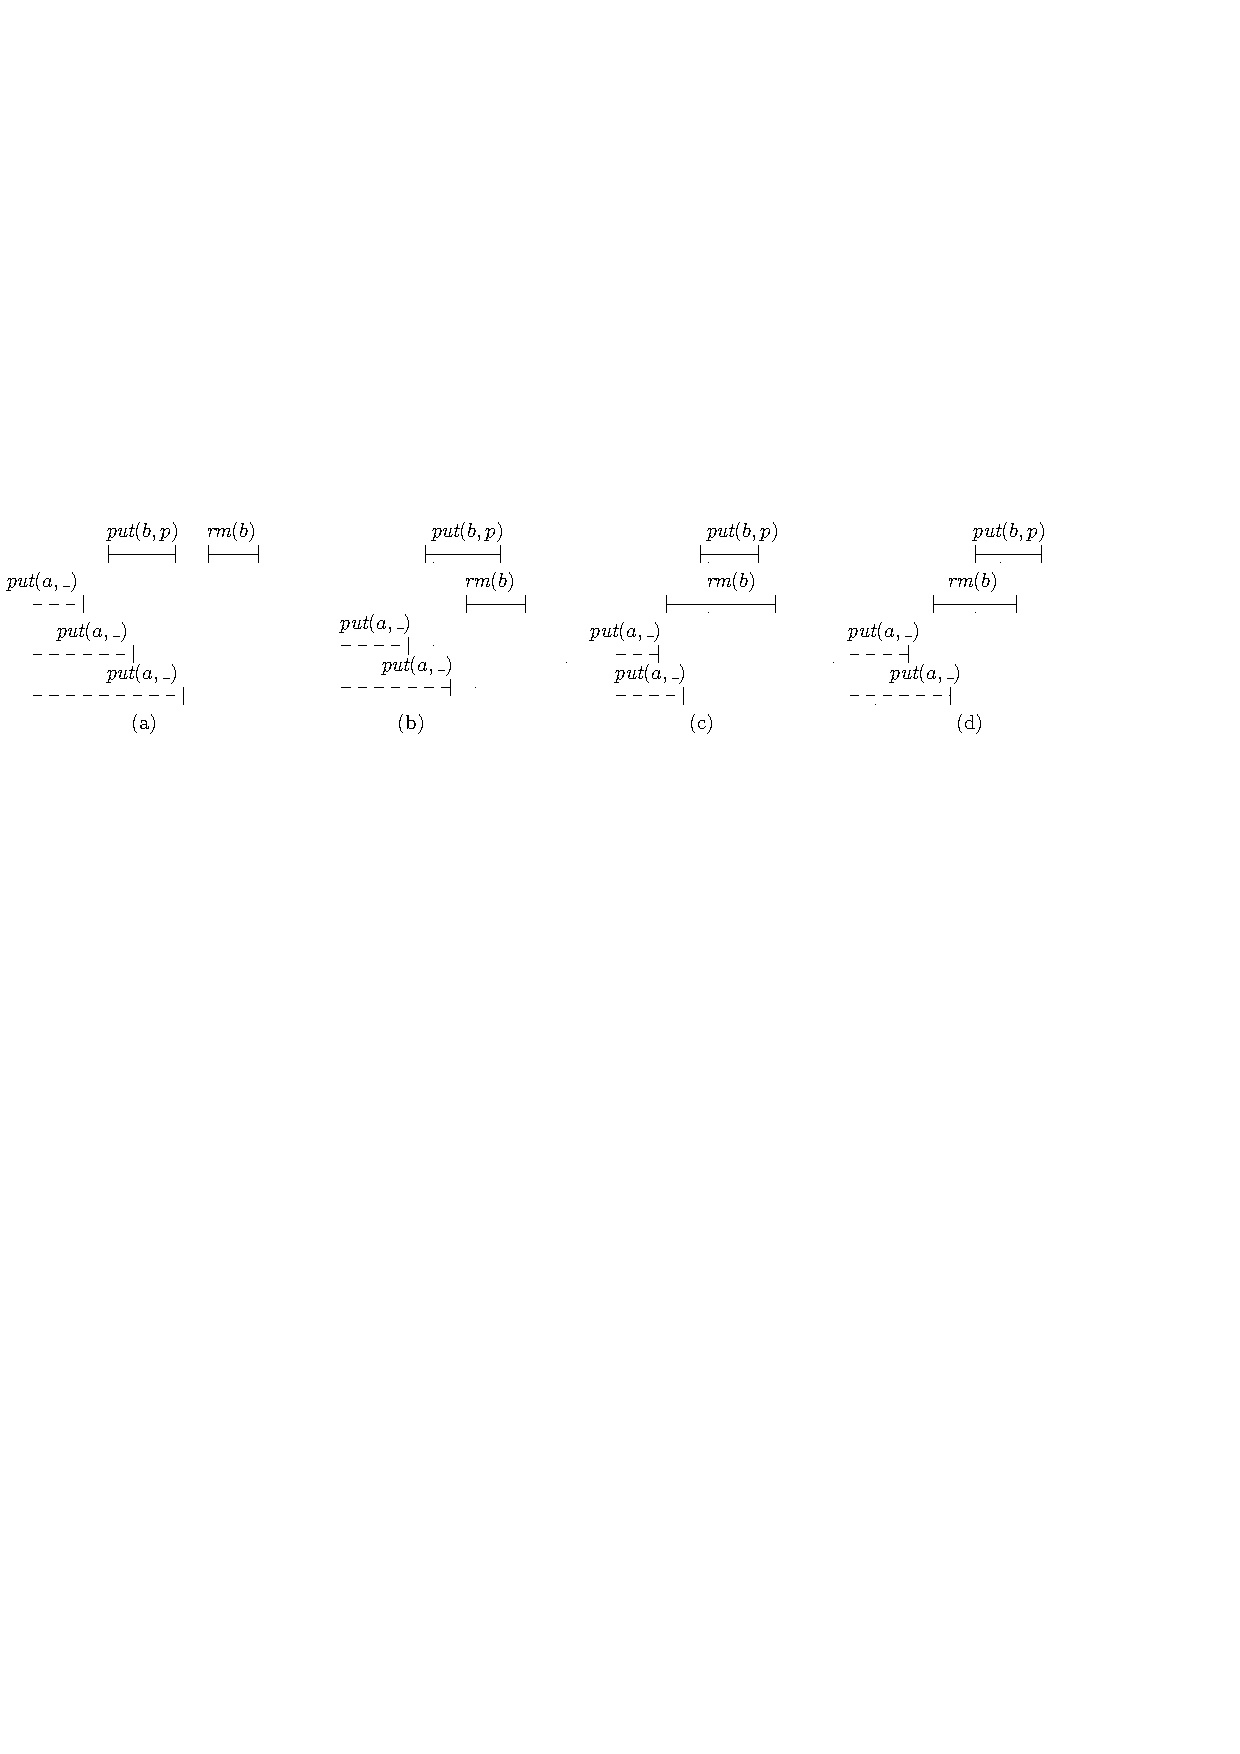
\includegraphics[width=.8\textwidth]{figures/PIC_HIS_PQ1Lar-fouCase.pdf}
  \caption{Orderings to be considered when defining a $\mathsf{MatchedMaxPriority}^>$-complete automaton.}
  \label{fig:executions APQ1Lar-1 in paper}
\end{figure}

\begin{figure}[t]
  \centering
  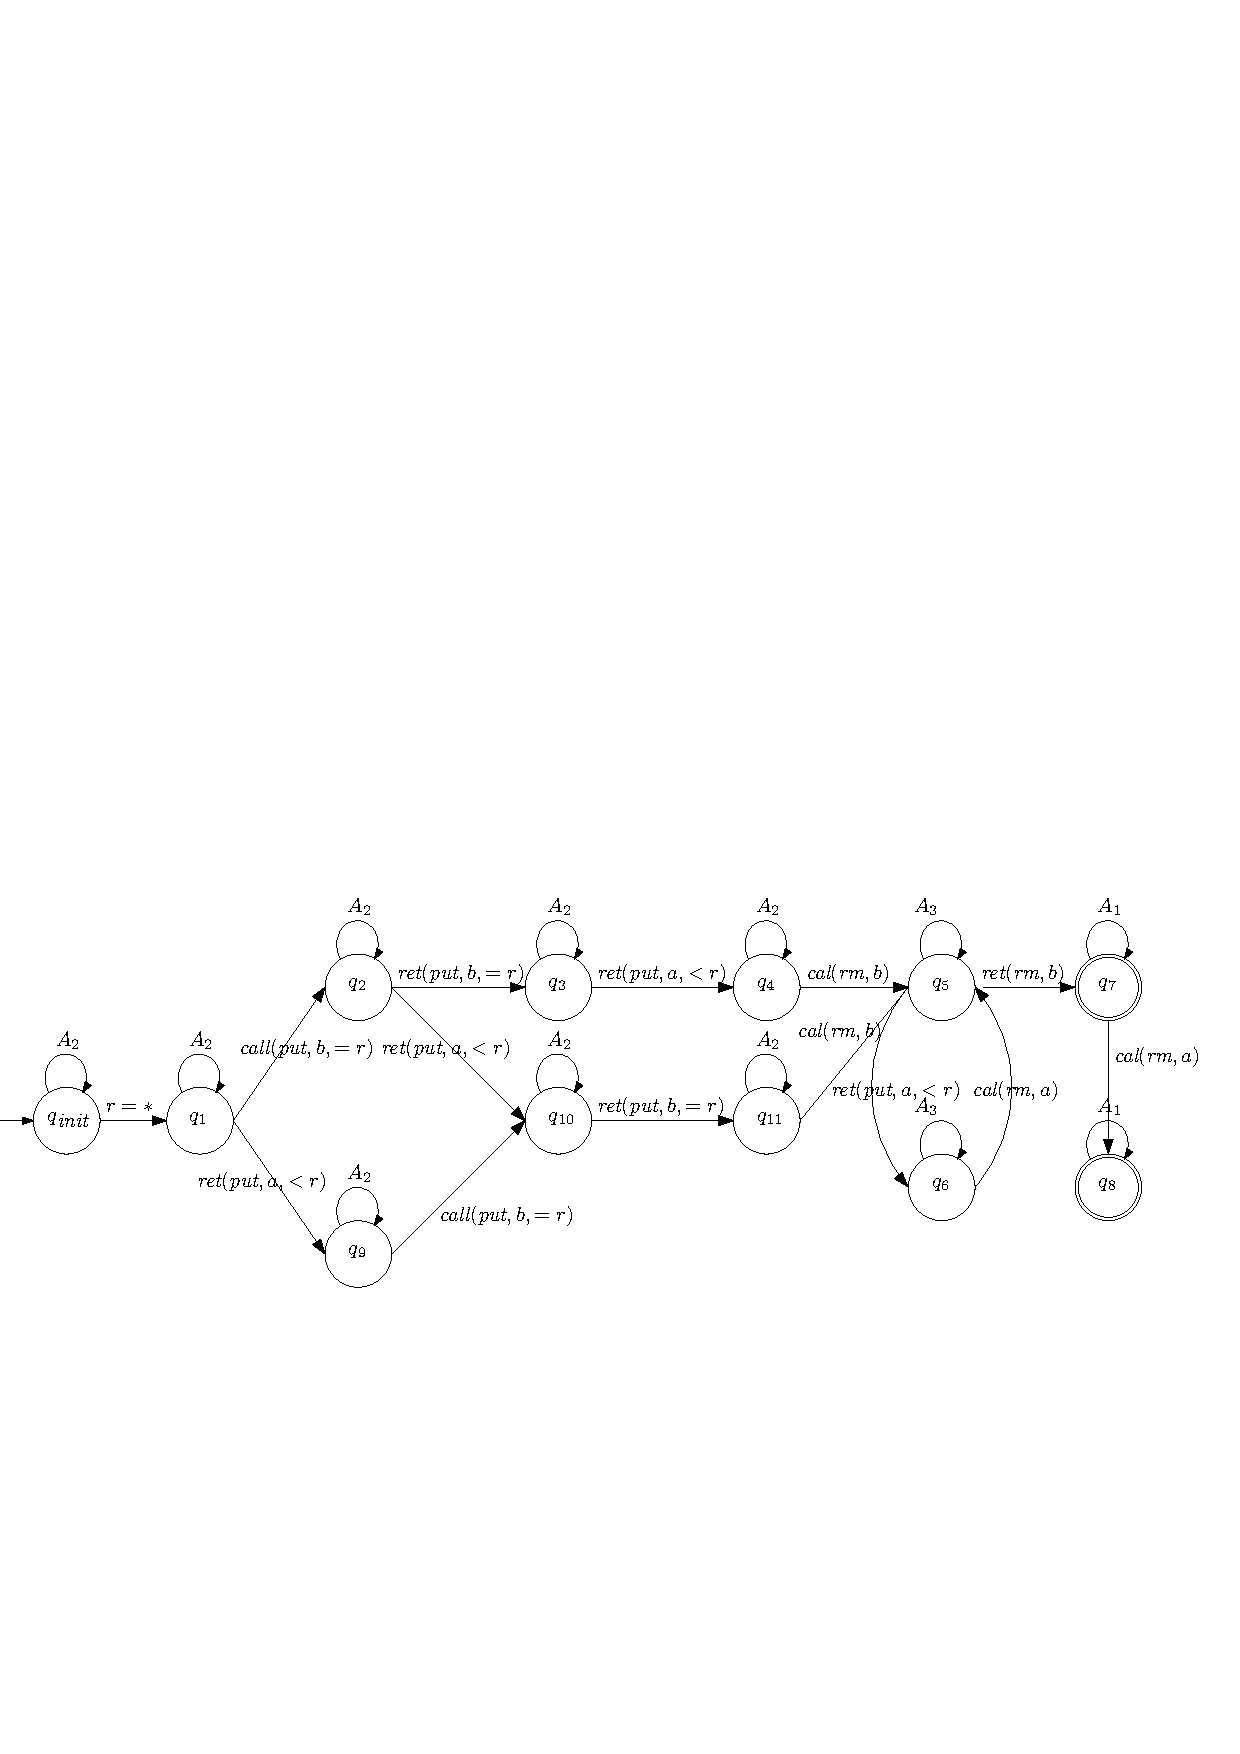
\includegraphics[width=.9\textwidth]{figures/PIC_AUTO_PQ1Lar-pprr.pdf}
  \caption{A register automaton capturing the scenario in Figure~\ref{fig:executions APQ1Lar-1 in paper}(a). We use the following notations: $A_1 = A \cup \{ \textit{ret}(\textit{rm},a) \}$, $A_2 = A \cup \{ \textit{call}(\textit{put},a,=r) \}$, $A_3 = A_2 \cup \{ \textit{ret}(\textit{rm},a) \}$, where $A = \{ \textit{call}(\textit{put},\top,\textit{true}),\textit{ret}(\textit{put},\top,\textit{true}), \textit{call}(\textit{rm},\top)$, $\textit{ret}(\textit{rm},\top),\textit{call}(\textit{rm},\textit{empty}),\textit{ret}(\textit{rm},\textit{empty}) \}$.}
  \label{fig:automata APQ1Lar-1 in paper}
\end{figure}





\subsubsection{A $\mathsf{MatchedMaxPriority}^=$-complete automaton}
\label{subsec:co-regular of EPQ1Equal}

When an execution contains at least two values of maximal priority, the acyclicity of the left-right constraints (for all the maximal priority values) is not enough to conclude that the execution is $\mathsf{MatchedMaxPriority}$-linearizable.
Intuitively, there may exist a value $a$ which is added before another value $b$ such that all the possible linearization points of $\textit{rm}(b)$ are disabled by the position of $\textit{rm}(a)$ in the happens-before. We give an example of such an execution $e$ in \figurename~\ref{fig:introduce pb order}, where $p_1\prec p_4$. This execution  is not linearizable w.r.t. $\mathsf{MatchedMaxPriority}$ (or $\mathsf{MatchedMaxPriority}^{=}$) even if
neither $a$ nor $b$ are covered by values with smaller priority.
Since $\textit{put}(a,p_4) <_{\textit{hb}} \textit{put}(b,p_4)$ and values of the same priority are removed in FIFO order, $\textit{rm}(a)$ should be linearized before $\textit{rm}(b)$ (i.e., this execution should be linearizable w.r.t. a sequence where $\textit{rm}(a)$ occurs before $\textit{rm}(b)$).
Since $\textit{rm}(b)$ cannot take effect during the interval of a smaller priority value, it could be only linearized in one of the two time intervals pictured with dotted lines in \figurename~\ref{fig:introduce pb order}. However, each of those time intervals ends before $\textit{call}(\textit{rm},a)$, and thus $\textit{rm}(a)$ cannot be linearized before $\textit{rm}(b)$.

\begin{figure}[t]
  \centering
  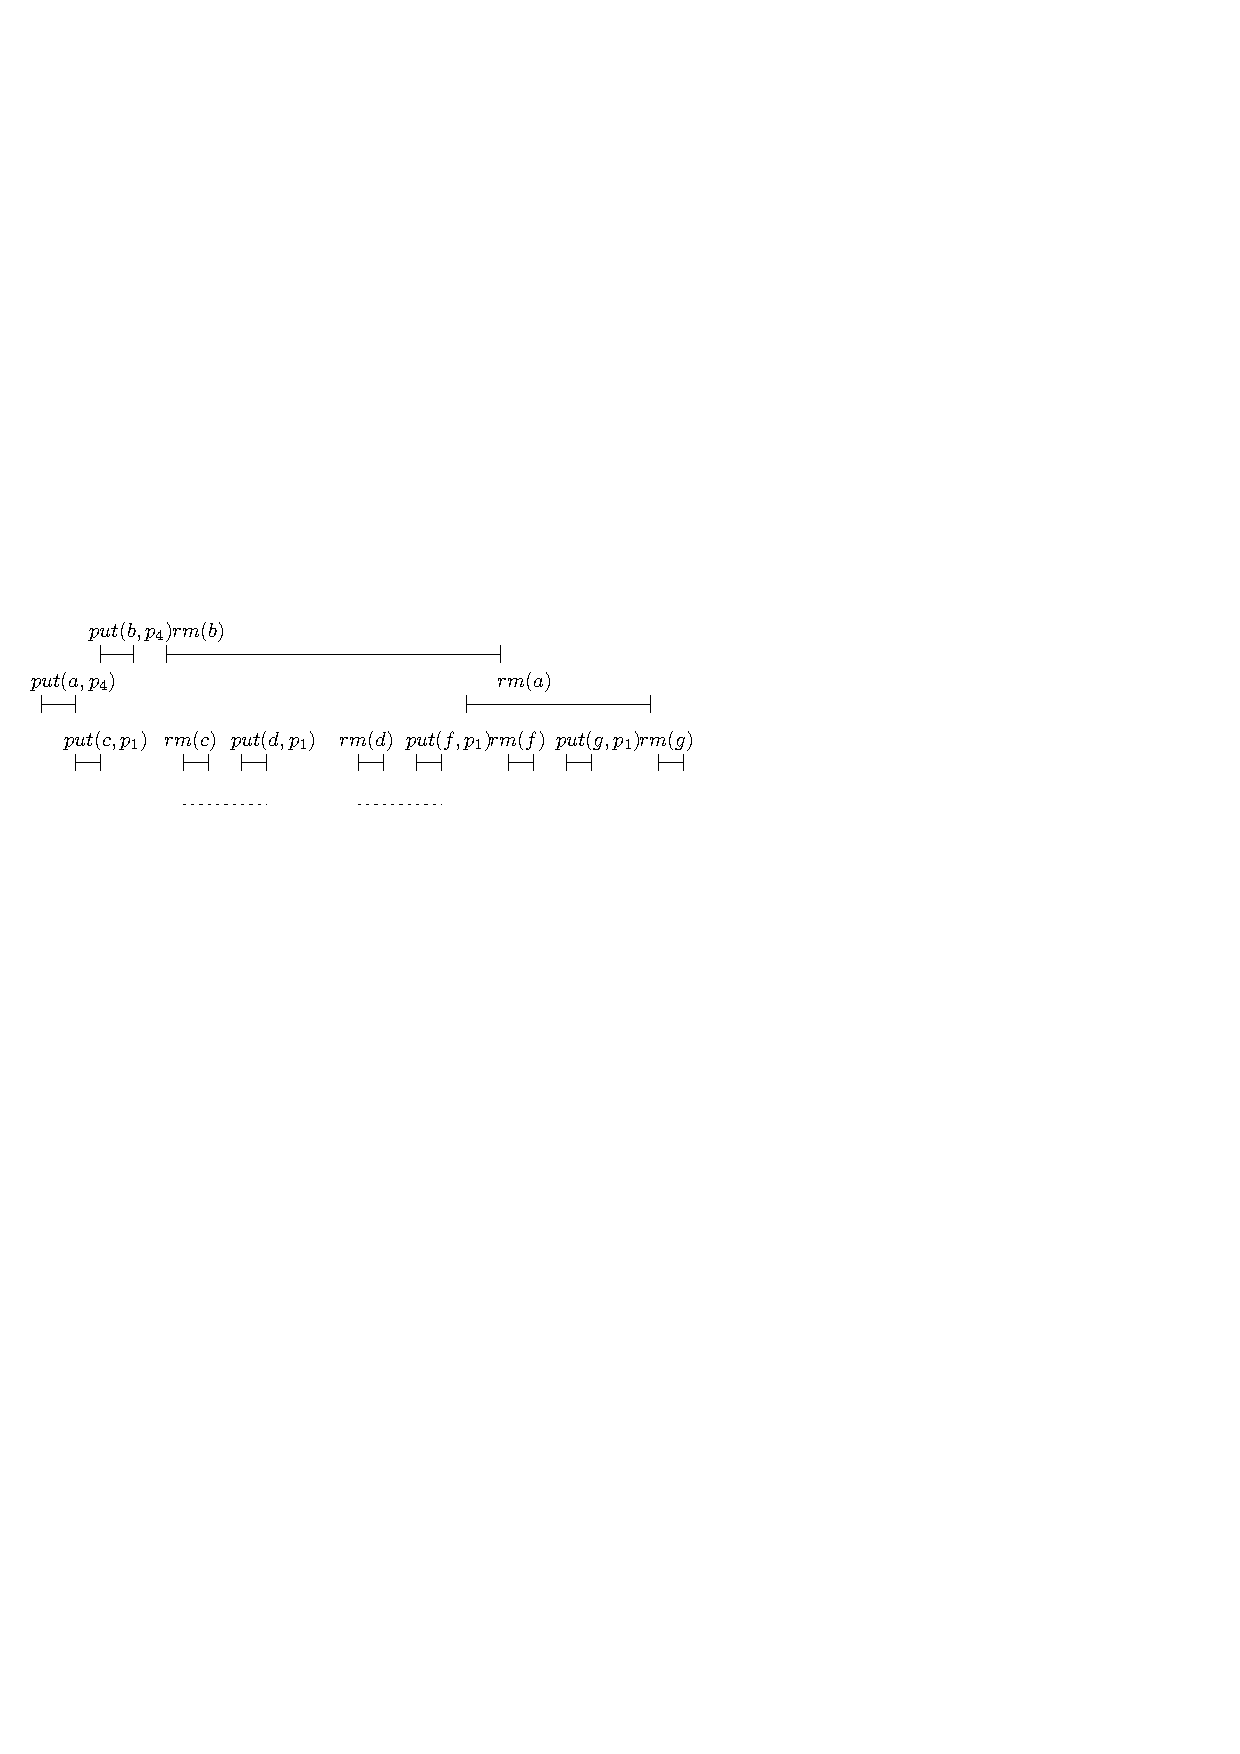
\includegraphics[width=0.5 \textwidth]{figures/PIC-HIS-INTRO-PB-ORDER-EPQ.pdf}
  \caption{An execution that is not $\mathsf{MatchedMaxPriority}^=$-linearizable.}
  \label{fig:introduce pb order}
\end{figure}

To recognize the scenarios in \figurename~\ref{fig:introduce pb order}, we introduce an order $<_{\textit{pb}}$ between values which intuitively, can be thought of as ``a value $a$ is put before another value $b$''.
More precisely, given a data-differentiated execution $e$ and two values $a$ and $b$ of maximal priority, $a <_{\textit{pb}} b$ if one of the following holds: (1) $\textit{put}(a,\_) <_{\textit{hb}} \textit{put}(b,\_)$, (2) $\textit{rm}(a) <_{\textit{hb}} \textit{rm}(b)$, or (3) $\textit{rm}(a) <_{\textit{hb}} \textit{put}(b,\_)$. Sometimes we use $a <_{\textit{pb}}^A b$, $a <_{\textit{pb}}^B b$, and $a <_{\textit{pb}}^C b$ to explicitly distinguish between these three cases. Let $<_{\textit{pb}}^*$ be the transitive closure of $<_{\textit{pb}}$.

To define the time intervals in which a remove like $\textit{rm}(b)$ in \figurename~\ref{fig:introduce pb order}, can be linearized (outside of intervals of smaller priority values) we use the notion of gap-point. As before, defining time intervals relies on an indexing of actions in an execution, starting with 0.

\begin{definition}\label{def:gap-point for matched put and rm operations}
Let $e$ be a data-differentiated execution with only one maximal priority $p$, and $\textit{put}(x,p)$ and $\textit{rm}(x)$ two operations in $e$. An index $i\in [0,|e|-1]$ is a \emph{gap-point of $x$} if $i$ is greater than or equal to the index of both $\textit{call}(\textit{put},x,p)$ and $\textit{call}(\textit{rm},x)$, smaller than the index of $\textit{ret}(\textit{rm},x)$, and not included in the interval of a value with priority smaller than $p$.
\end{definition}

The case of \figurename~\ref{fig:introduce pb order} can be formally described as follows: $a <_{\textit{pb}}^* b$ while the right-most gap-point of $b$ is before $\textit{call}(\textit{rm},a)$ or $\textit{call}(\textit{put},a,p_4)$. The following lemma states that these conditions are enough to characterize non-linearizability w.r.t. $\mathsf{MatchedMaxPriority}^{=}$. It is proved in Appendix~\ref{sec:appendix proof and definition in section co-regular of EPQ1Equal}. 

\begin{lemma}
\label{lemma:EPQ1Equal as pb order and gap-point}
Let $e$ be a data-differentiated execution with only one maximal priority $p$ such that $\mathsf{Has\text{-}MatchedMaxPriority}(e)$ holds.
Then, $e$ is not $\mathsf{MatchedMaxPriority}^{=}$-linearizable iff $e$ contains two values $x$ and $y$ of maximal priority $p$ such that $y <_{\textit{pb}}^* x$, and the rightmost gap-point of $x$ is strictly smaller than the index of $\textit{call}(\textit{put},y,p)$ or $\textit{call}(\textit{rm},y)$.
\end{lemma}


The following shows that the number of values needed to witness that $y <_{\textit{pb}}^* x$, for some $x$ and $y$, is bounded.

\begin{lemma}
\label{lemma:ob order has bounded length}
Let $e$ be a data-differentiated execution such that $a <_{\textit{pb}} a_1 <_{\textit{pb}} \ldots <_{\textit{pb}} a_m <_{\textit{pb}} b$ holds for some set of values $a$, $a_1$,$\ldots$,$a_m$, $b$. Then, one of the following holds:
\begin{itemize}
\item[-] $a <_{\textit{pb}}^A b$, $a <_{\textit{pb}}^B b$, or $a <_{\textit{pb}}^C b$,

\item[-] $a <_{\textit{pb}}^A a_i <_{\textit{pb}}^B b$ or $a <_{\textit{pb}}^B a_i <_{\textit{pb}}^A b$, for some $i$.
\end{itemize}
\end{lemma}

\begin{figure}[t]
  \centering
  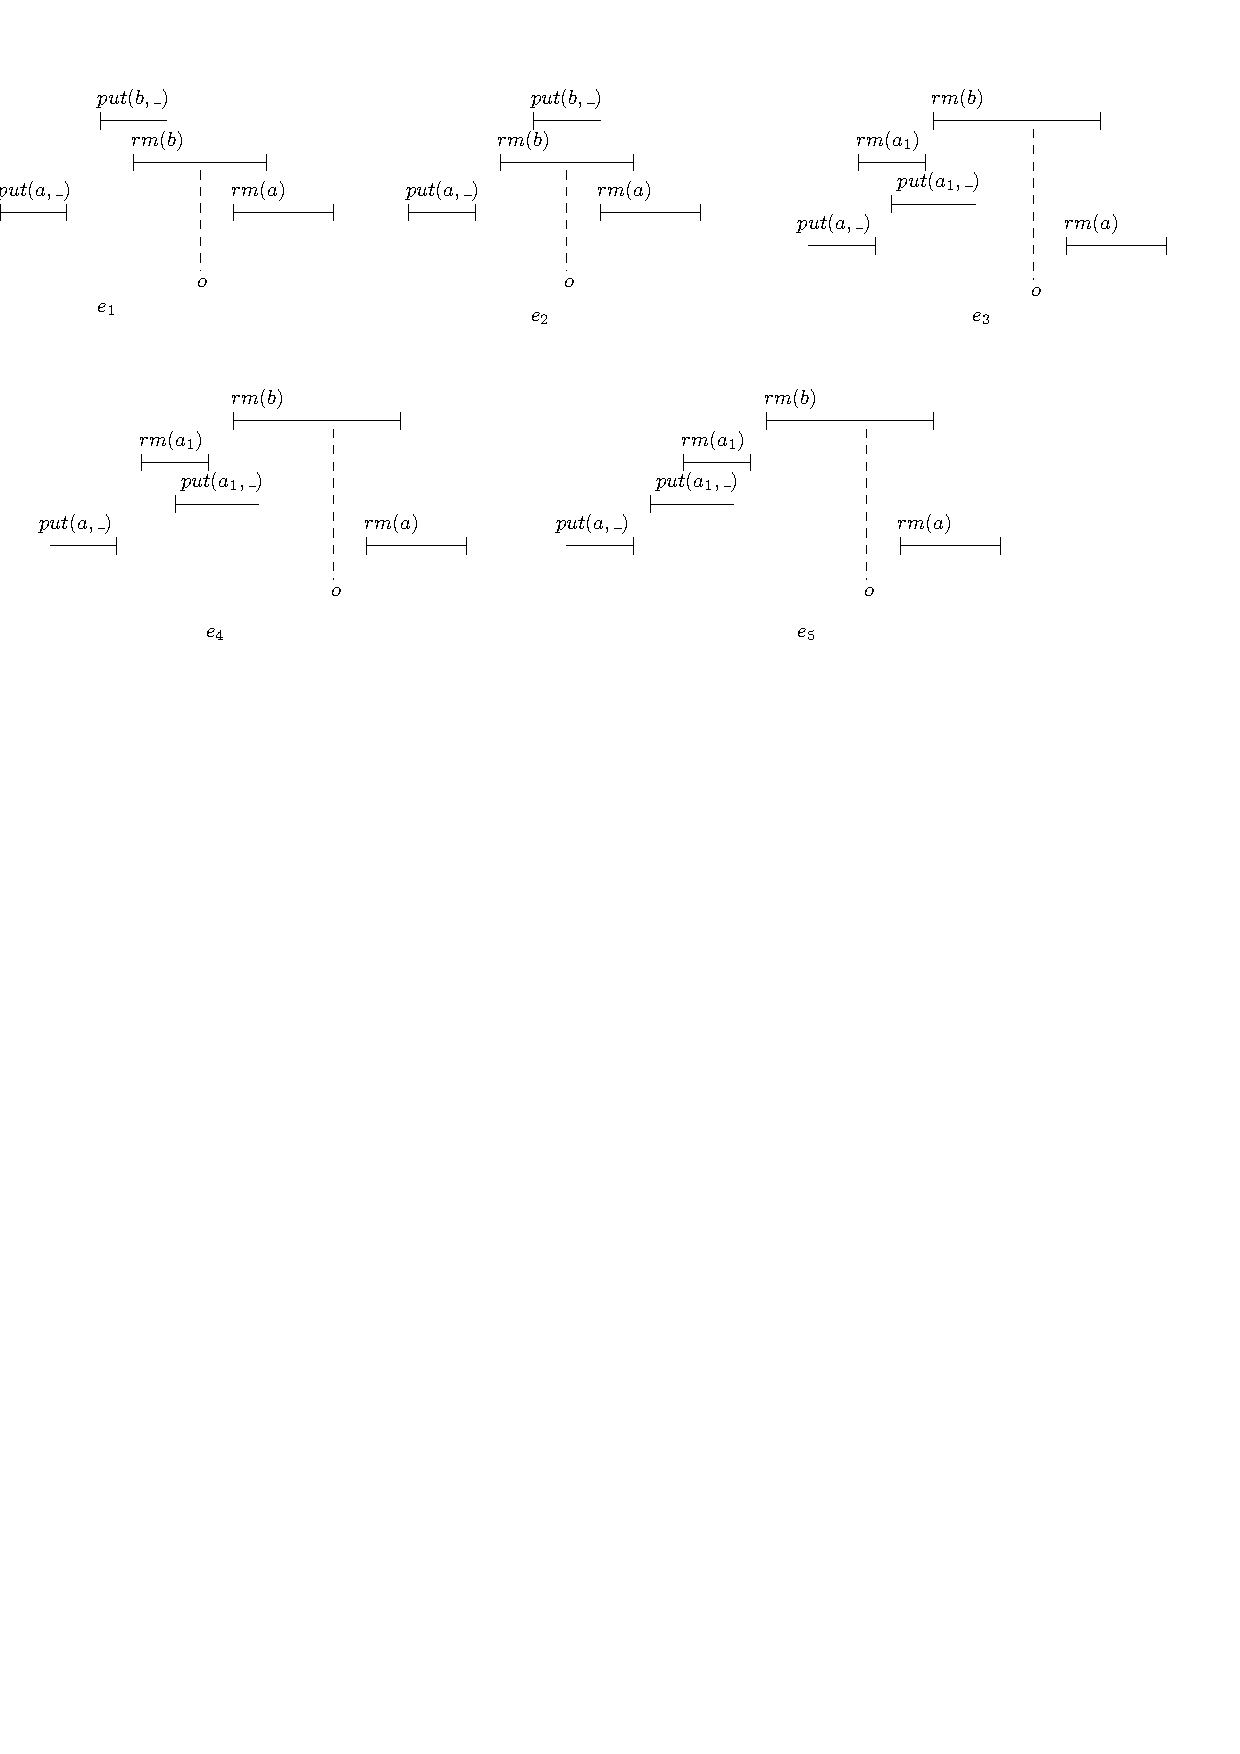
\includegraphics[width=0.8 \textwidth]{figures/PIC-HIS-FiveEnumerations.pdf}
  \caption{Orderings to be considered when defining a $\mathsf{MatchedMaxPriority}^=$-complete automaton. We omit the operations which can be ordered arbitrarily, e.g., $\textit{put}(b)$ in the cases (d) and (e).}
  \label{fig:five enumerations}
\end{figure}

To characterize violations to $\mathsf{MatchedMaxPriority}^{=}$-linearizability, one has to consider all the possible orders between call/return actions of the operations on values $a$, $b$, and $a_i$ in Lemma \ref{lemma:ob order has bounded length}, and the right-most gap point of $b$. Excluding the inconsistent cases, we are left with the five orders in \figurename~\ref{fig:five enumerations}, where $o$ denotes the rightmost gap-point of $b$ (see Lemma \ref{lemma:five enumeration is enough for EPQ1Equal} in Appendix~\ref{sec:appendix proof and definition in section co-regular of EPQ1Equal}).
For each case, we define an automaton recognizing the induced set of violations. The register automaton for the case in \figurename~\ref{fig:five enumerations}(a) is shown in \figurename~\ref{fig:an enumeration and its witness automaton}. In this case, Lemma~\ref{lemma:EPQ1Equal as pb order and gap-point} is equivalent to the fact that intuitively, the time interval from $\textit{call}(\textit{rm},a)$ to $\textit{ret}(\textit{rm},b)$ is covered by lower priority values (thus, there is no gap-point of $b$ which occurs after $\textit{call}(\textit{rm},a)$). By data-independence, these lower priority values can be renamed to a fixed value $c$. In Appendix~\ref{sec:appendix proof and definition in section co-regular of EPQ1Equal}, we give the detailed construction for register automata for all five orders in \figurename~\ref{fig:five enumerations}. 


\begin{figure}[t]
  \centering
  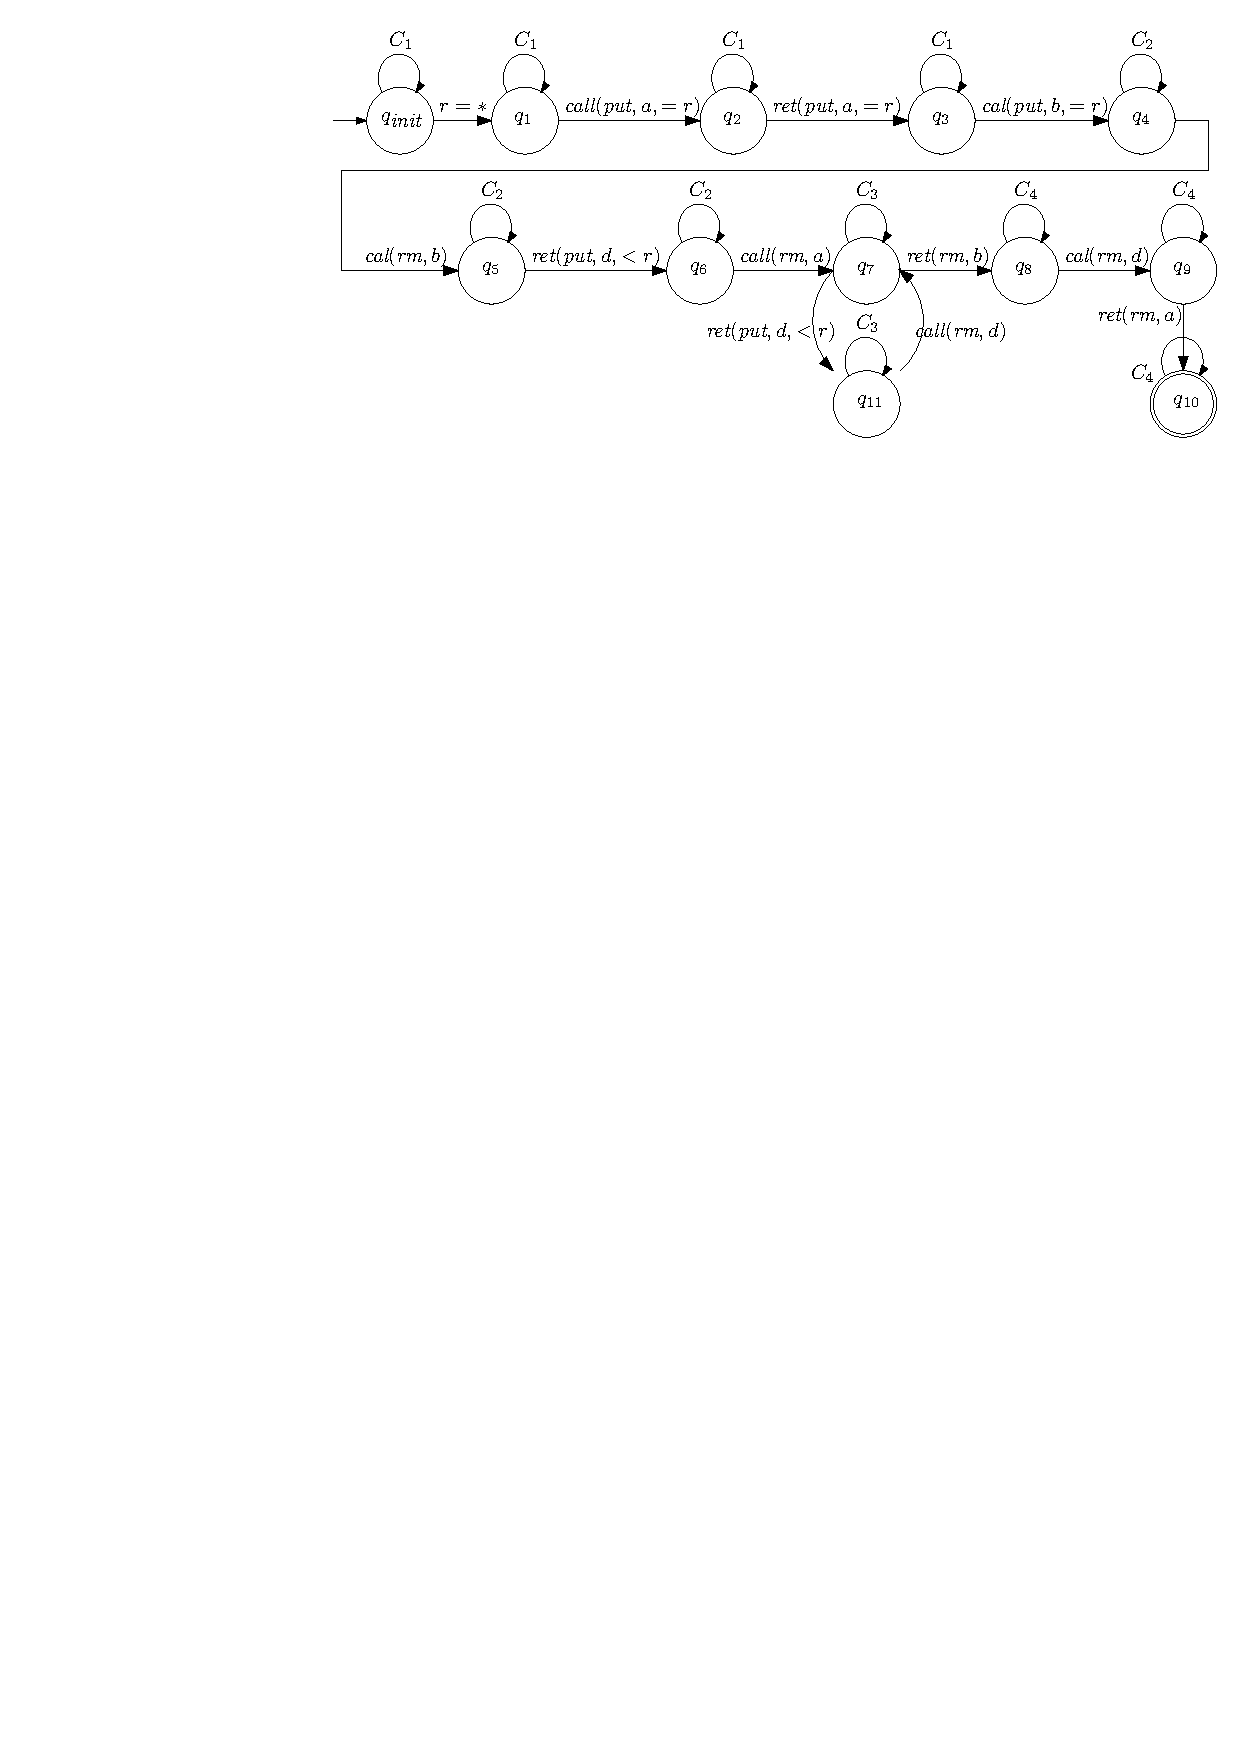
\includegraphics[width=0.65 \textwidth]{figures/PIC-WitnessAutomata-For1.pdf}
  \caption{A register automaton for the case in Figure~\ref{fig:five enumerations}(a), where $A_1 = A \cup \{ \textit{call}(\textit{put},c,<r)\}$, $A_2 = A_1 \cup \{ \textit{ret}(\textit{put},b,=r) \}$, $A_3 = A_2 \cup \{ \textit{ret}(\textit{rm},c) \}$, $A_4 = A \cup \{ \textit{ret}(\textit{put},b,=r), \textit{ret}(\textit{rm},c) \}$, where $A = \{ \textit{call}(\textit{put},\top,\textit{true})$,$\textit{ret}(\textit{put},\top,\textit{true})$,$\textit{call}(\textit{rm},\top)$,$\textit{ret}(\textit{rm},\top)$,$\textit{call}(\textit{rm},\textit{empty})$,$\textit{ret}(\textit{rm},\textit{empty})\}$.}
  \label{fig:an enumeration and its witness automaton}
\end{figure}



\subsection{Decidability Result}
\label{subsec:combine step-by-step linearizability and co-regular}

We describe a class $\mathcal{C}$ of data-independent implementations for which linearizability w.r.t. $\seqPQ$ is decidable. The implementations in $\mathcal{C}$ allow an unbounded number of values but a bounded number of priorities. Each method has a finite set of local variables storing Boolean values or values from $\mathbb{D}$. Methods communicate through a finite number of shared variables interpreted also as Booleans or values from $\mathbb{D}$. To ensure data independence, values in $\mathbb{D}$ may be assigned, but never used in Boolean expressions (e.g., of if-then-else statements). This class captures typical implementations, or finite-state abstractions thereof, e.g., obtained via predicate abstraction. The $\Gamma$-complete automata we define use a fixed set $D=\{a,b,c,a_1,\top\}$ of values ($a_1$ is needed to deal with the second item in Lemma~\ref{lemma:ob order has bounded length}). Therefore, for any $\Gamma$, $\mathcal{C}\cap A(\Gamma)\neq\emptyset$ iff $\mathcal{C}_D\cap A(\Gamma)\neq\emptyset$, where $\mathcal{C}_D$ is the subset of $\mathcal{C}$ that uses only values in $D$.

The set of executions $\mathcal{C}_D$ can be represented by a Vector Addition System with States (VASS). Since the set of values and priorities is bounded, each method invocation can be represented by a finite-state automaton (see~\cite{conf/esop/BouajjaniEEH13}). For a fixed set of priorities $P\subseteq \mathbb{P}$, the register automata $A(\Gamma)$ can be transformed to finite-state automata (the number of valuations of the registers is bounded). Thus, checking linearizability of an implementation in $\mathcal{C}$ is PSPACE when the number of threads is bounded, and EXPSPACE, otherwise. Moreover, reachability in VASSs can be reduced to checking linearizability of such an implementation. Essentially, given an instance of the VASS reachability problem, one can define a priority queue implementation where the $\textit{put}$ methods behave correctly and additionally, they include the code of the VASS simulation defined in~\cite{conf/esop/BouajjaniEEH13}, and the $\textit{rm}$ methods behave correctly, except for the moment where the target state is reached, in which case they trigger a linearizability violation by returning an arbitrary value. 

Based on above discussion, we have the following complexity result. The detailed proof can be found in Appendix \ref{subsec:appendix proof and definition in subsection decidability result}.

%\begin{restatable}{theorem}{ComplexityOfPriorityQueue}
%\label{theorem:complexity of priority queue}
%Verifying whether an implementation in $\mathcal{C}$ is linearizable w.r.t. $\seqPQ$ is PSPACE-complete for a fixed number of %threads, and EXPSPACE-complete otherwise.
%\end{theorem}



\begin{theorem}
\label{theorem:complexity of priority queue}
Verifying whether an implementation in $\mathcal{C}$ is linearizable w.r.t. $\seqPQ$ is PSPACE-complete for a fixed number of threads, and EXPSPACE-complete otherwise.
\end{theorem}








